\documentclass[letterpaper,12pt]{article}
\usepackage{tabularx}
\usepackage{amsmath}
\usepackage{graphicx}
\usepackage[margin=1in,letterpaper]{geometry}
\usepackage{cite}
\usepackage{float}
\usepackage[final]{hyperref}
\hypersetup{
    colorlinks=true,
    linkcolor=blue,
    citecolor=blue,
    filecolor=magenta,
    urlcolor=blue
}

\begin{document}

\title{{{ title }}}
\author{{{ author }}}
\date{{{ date }}}
\maketitle

\begin{abstract}
{{ abstract }}

\begin{table}[H]
\begin{center}
\caption{Summary Results}
\label{tbl:issues}
\begin{tabular}{|c|c|c|}
\hline
\textbf{Variable} & \textbf{Value} & \textbf{Unit} \\
\hline
Ambient Temperature &  & C \\
\hline
Average Fill Pressure &  & psi \\
\hline
Fill Time &  & s \\
\hline
Peak Run Pressure &  & psi \\
\hline
Peak CC Pressure &  & psi \\
\hline
Peak Tank Pressure &  & psi \\
\hline
Time To Peak Tank Pressure &  & s \\
\hline
Burn Time For Hotfire &  & s \\
\hline
Peak Thrust &  & N \\
\hline
Total Impulse &  & Ns \\
\hline
Tank Mass (measured) &  &  \\
\hline
Tank Mass (estimated) &  &  \\
\hline
\end{tabular}
\end{center}
\end{table}

\end{abstract}

\section{Plots}

\begin{figure}[H]
    \centering
    \includegraphics[width=0.7\textwidth]{tank_fill_pressure_drop.png}
    \caption{Caption of the figure}
    \label{fig:labelname}
\end{figure}

\begin{figure}[H]
    \centering
    \includegraphics[width=0.7\textwidth]{temp.png}
    \caption{Caption of the figure}
    \label{fig:labelname}
\end{figure}

\begin{figure}[H]
    \centering
    \includegraphics[width=0.7\textwidth]{tank_run_pressure_drop.png}
    \caption{Caption of the figure}
    \label{fig:labelname}
\end{figure}

\begin{figure}[H]
    \centering
    \includegraphics[width=0.7\textwidth]{run_cc_pressure_drop.png}
    \caption{Caption of the figure}
    \label{fig:labelname}
\end{figure}

\begin{figure}[H]
    \centering
    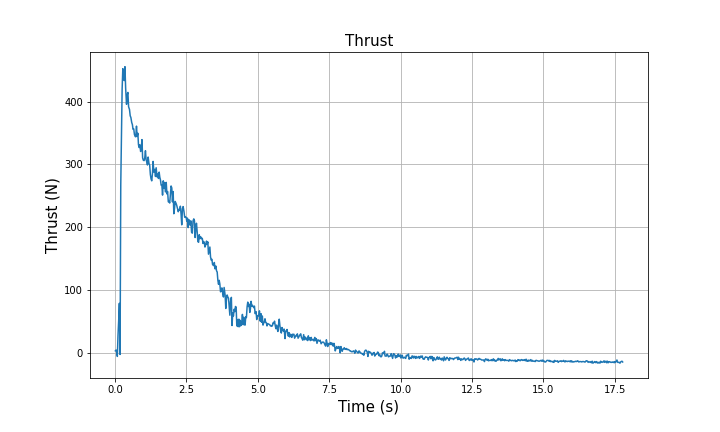
\includegraphics[width=0.7\textwidth]{thrust.png}
    \caption{Caption of the figure}
    \label{fig:labelname}
\end{figure}

\begin{figure}[H]
    \centering
    \includegraphics[width=0.7\textwidth]{mass.png}
    \caption{Caption of the figure}
    \label{fig:labelname}
\end{figure}

\begin{figure}[H]
    \centering
    \includegraphics[width=0.7\textwidth]{mass_flow_rate.png}
    \caption{Caption of the figure}
    \label{fig:labelname}
\end{figure}

\section{Analysis}
Specific analysis of hotfire data to determine whether the specific goal was met

\section{Issues Encountered}
\begin{table}[H]
\begin{center}
\caption{Issues Encountered}
\label{tbl:issues}
\begin{tabular}{|c|c|c|}
\hline
\textbf{Issue} & \textbf{Reason} & \textbf{Resolution} \\
\hline

\hline
\end{tabular}
\end{center}
\end{table}

\section{Conclusions}
{{ conclusions }}


\end{document}